% Dummy comment so that files shows up in Reviewable.
Recall that in Section~\ref{sec:unconstrained_convex_formulation}
we defined \emph{Inverse Dynamics}
as the construction of the optimal dual impulses
from the optimal primal velocities.  As shown in~\cite{bib:todorov2014},
these impulses have formula $\bgamma = P_{\mathcal{F}}(\vf{y})$, 
where $P_{\mathcal{F}}$ denotes projection
with respect to the weighted norm $\|\cdot\|_{\mf R}$, i.e.,
\[
P_{\mathcal{F}}(\mf{y}) = \argmin_{\bgamma\in\mathcal{F}} \quad \frac{1}{2}(\bgamma-\mf{y})^T\vf{R}(\bgamma-\mf{y}).
\]
We next show this projection is easily computed
if one first applies a change of variables and works with the usual Euclidean norm $\|\cdot\|$.

Given the separable structure of the problem, projection of $\mf{y}$ onto $\mathcal{F} =
\mathcal{F}_{1} \times \mathcal{F}_{2} \cdots
\mathcal{F}_{{n-1}}\times\mathcal{F}_{n}$ can be done by projecting $\vf{y}_i$ onto each
cone $\mathcal{F}_{i}$ individually. To ease notation, we drop the contact subindex $i$ and we consider a diagonal regularization of the form $\vf{R} = \text{diag}([R_t, R_t, R_n])$.

To begin, we let $\tilde{\bgamma}=\vf{R}^{1/2}\bgamma$ and
$\tilde{\vf{y}}=\vf{R}^{1/2}\vf{y}$ to rewrite $P_{\mathcal{F}}(\vf{y})$ as
\[
  P_{\mathcal{F}}(\vf{y}) = \mf{R}^{-1/2} \argmin_{\tilde \bgamma\in \mf{R}^{1/2} \mathcal{F}} \frac{1}{2}\Vert\tilde\bgamma-\tilde{\vf{y}} \Vert_2^2
\]                                                                               
Observing that $\mf{R}^{1/2} \mathcal{F} = \tilde{\mathcal{F}}$ for $\tilde \mu =\mu\,(R_t/R_n)^{1/2}$,
we conclude that
\begin{eqnarray}
  P_\mathcal{F}(\vf{y})=\vf{R}^{-1/2} P_{\tilde{\mathcal{F}}}(\tilde{\vf{y}})
	\label{eq:local_optimization_problem_tilde}
\end{eqnarray}
where $P_{\tilde{\mathcal{F}}} : \mathbb{R}^3 \rightarrow \mathbb{R}^3$ denotes Euclidean projection onto $\tilde{\mathcal{F}}$.

A simple piecewise formula for evaluating $P_{\tilde{\mathcal{F}}}$ is obtained
by partitioning its domain  into three regions, shown in Fig. \ref{fig:cone_regions}. This partition consists of the
closed cone $\tilde{\mathcal{F}}$, denoted with $\mathcal{R}_I$, the interior of the
polar $\tilde{\mathcal{F}}^\circ$, denoted with $\mathcal{R}_{III}$, and the
remaining area, which we denote with $\mathcal{R}_{II}$. For $\tilde{\vf{y}}\in\mathcal{R}_I$ we simply have
that $P_{\tilde{\mathcal{F}}}(\tilde{\vf{y}}) = \tilde{\vf{y}}$. When $\tilde{\vf{y}}\in\mathcal{R}_{III}$,
$P_{\tilde{\mathcal{F}}}(\tilde{\vf{y}}) = \vf{0}$. Finally, when $\tilde{\vf{y}}\in\mathcal{R}_{II}$, we
evaluate $P_{\tilde{\mathcal{F}}}(\tilde{\vf{y}})$ via Euclidean projection onto
the boundary of $\tilde{\mathcal{F}}$, which admits a simple formula. We define
$\hat{\vf{f}}=[\tilde{\mu}\hat{\vf{t}}, 1]/\sqrt{1+\tilde{\mu}^2}$ the unit
vector along the wall of the cone shown in Fig. \ref{fig:cone_regions}, with
$\hat{\vf{t}}=\tilde{\vf{y}}_t/\Vert\tilde{\vf{y}}_t\Vert=\vf{y}_t/\Vert\vf{y}_t\Vert$. Then the projection is computed as
$\tilde{\bgamma}=(\tilde{\vf{y}}\cdot\hat{\vf{f}})\hat{\vf{f}}$. After some algebraic manipulation we have that 
$P_{\tilde{\mathcal{F}}}(\tilde{\vf{y}}) = [\tilde{\bgamma}_t, \tilde{\gamma}_n]$,
where
\begin{align}\label{eq:ProjectionFormula}
\begin{aligned}
  \tilde{\bgamma}_t       &= \tilde{\mu}\tilde{\gamma}_n\hat{\vf{t}}\\
        \tilde{\gamma}_n  &= \frac{1}{1+\tilde{\mu}^2}\left(\tilde{y}_n +
	\tilde{\mu}\tilde{y}_r\right)
\end{aligned}
\end{align}
where $\tilde{y}_r=\Vert\tilde{\vf{y}}_t\Vert$. Note that this formula is
well-defined on $\mathcal{R}_{II}$, since $\vf{y}_t = \vf{0}$ only if $\vf{y}$ is lies in regions $\mathcal{R}_{I}$ or $\mathcal{R}_{III}$.
\begin{figure}[!h]
    \centering
    %\vspace{6pt}
    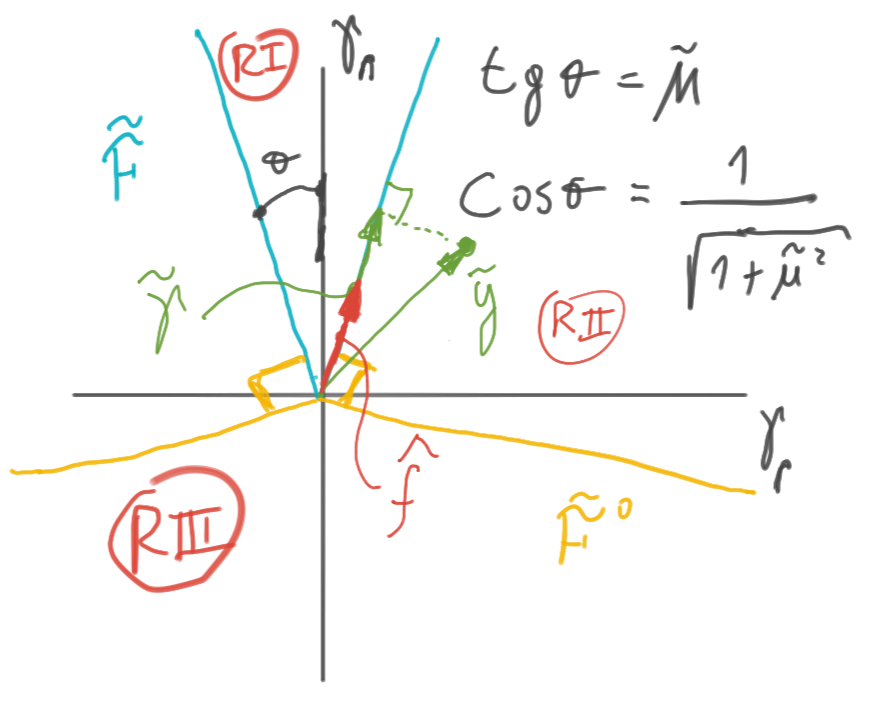
\includegraphics[width=0.45\columnwidth]{figures/cone_regions.png}
    \caption{Geometry of $\tilde{\mathcal{F}}$ and regions in the
    $\tilde{\vf{y}}$ space.\RedHighlight{No need to define $\theta$, the text does not use it.}}
    \label{fig:cone_regions}
\end{figure}

Finally, we apply the inverse transformation
$\bgamma=\mf{R}^{-1/2}P_{\tilde{\mathcal{F}}}(\tilde{\vf{y}})$ and after some
algebraic manipulation we recover the projection $\bgamma =
P_\mathcal{F}(\vf{y})$ in Eq. \eqref{eq:analytical_y_projection}.


